% Options for packages loaded elsewhere
% Options for packages loaded elsewhere
\PassOptionsToPackage{unicode}{hyperref}
\PassOptionsToPackage{hyphens}{url}
\PassOptionsToPackage{dvipsnames,svgnames,x11names}{xcolor}
%
\documentclass[
  number]{elsarticle}
\usepackage{xcolor}
\usepackage{amsmath,amssymb}
\setcounter{secnumdepth}{5}
\usepackage{iftex}
\ifPDFTeX
  \usepackage[T1]{fontenc}
  \usepackage[utf8]{inputenc}
  \usepackage{textcomp} % provide euro and other symbols
\else % if luatex or xetex
  \usepackage{unicode-math} % this also loads fontspec
  \defaultfontfeatures{Scale=MatchLowercase}
  \defaultfontfeatures[\rmfamily]{Ligatures=TeX,Scale=1}
\fi
\usepackage{lmodern}
\ifPDFTeX\else
  % xetex/luatex font selection
\fi
% Use upquote if available, for straight quotes in verbatim environments
\IfFileExists{upquote.sty}{\usepackage{upquote}}{}
\IfFileExists{microtype.sty}{% use microtype if available
  \usepackage[]{microtype}
  \UseMicrotypeSet[protrusion]{basicmath} % disable protrusion for tt fonts
}{}
\makeatletter
\@ifundefined{KOMAClassName}{% if non-KOMA class
  \IfFileExists{parskip.sty}{%
    \usepackage{parskip}
  }{% else
    \setlength{\parindent}{0pt}
    \setlength{\parskip}{6pt plus 2pt minus 1pt}}
}{% if KOMA class
  \KOMAoptions{parskip=half}}
\makeatother
% Make \paragraph and \subparagraph free-standing
\makeatletter
\ifx\paragraph\undefined\else
  \let\oldparagraph\paragraph
  \renewcommand{\paragraph}{
    \@ifstar
      \xxxParagraphStar
      \xxxParagraphNoStar
  }
  \newcommand{\xxxParagraphStar}[1]{\oldparagraph*{#1}\mbox{}}
  \newcommand{\xxxParagraphNoStar}[1]{\oldparagraph{#1}\mbox{}}
\fi
\ifx\subparagraph\undefined\else
  \let\oldsubparagraph\subparagraph
  \renewcommand{\subparagraph}{
    \@ifstar
      \xxxSubParagraphStar
      \xxxSubParagraphNoStar
  }
  \newcommand{\xxxSubParagraphStar}[1]{\oldsubparagraph*{#1}\mbox{}}
  \newcommand{\xxxSubParagraphNoStar}[1]{\oldsubparagraph{#1}\mbox{}}
\fi
\makeatother


\usepackage{longtable,booktabs,array}
\usepackage{calc} % for calculating minipage widths
% Correct order of tables after \paragraph or \subparagraph
\usepackage{etoolbox}
\makeatletter
\patchcmd\longtable{\par}{\if@noskipsec\mbox{}\fi\par}{}{}
\makeatother
% Allow footnotes in longtable head/foot
\IfFileExists{footnotehyper.sty}{\usepackage{footnotehyper}}{\usepackage{footnote}}
\makesavenoteenv{longtable}
\usepackage{graphicx}
\makeatletter
\newsavebox\pandoc@box
\newcommand*\pandocbounded[1]{% scales image to fit in text height/width
  \sbox\pandoc@box{#1}%
  \Gscale@div\@tempa{\textheight}{\dimexpr\ht\pandoc@box+\dp\pandoc@box\relax}%
  \Gscale@div\@tempb{\linewidth}{\wd\pandoc@box}%
  \ifdim\@tempb\p@<\@tempa\p@\let\@tempa\@tempb\fi% select the smaller of both
  \ifdim\@tempa\p@<\p@\scalebox{\@tempa}{\usebox\pandoc@box}%
  \else\usebox{\pandoc@box}%
  \fi%
}
% Set default figure placement to htbp
\def\fps@figure{htbp}
\makeatother





\setlength{\emergencystretch}{3em} % prevent overfull lines

\providecommand{\tightlist}{%
  \setlength{\itemsep}{0pt}\setlength{\parskip}{0pt}}



 


\makeatletter
\@ifpackageloaded{caption}{}{\usepackage{caption}}
\AtBeginDocument{%
\ifdefined\contentsname
  \renewcommand*\contentsname{Table of contents}
\else
  \newcommand\contentsname{Table of contents}
\fi
\ifdefined\listfigurename
  \renewcommand*\listfigurename{List of Figures}
\else
  \newcommand\listfigurename{List of Figures}
\fi
\ifdefined\listtablename
  \renewcommand*\listtablename{List of Tables}
\else
  \newcommand\listtablename{List of Tables}
\fi
\ifdefined\figurename
  \renewcommand*\figurename{Figure}
\else
  \newcommand\figurename{Figure}
\fi
\ifdefined\tablename
  \renewcommand*\tablename{Table}
\else
  \newcommand\tablename{Table}
\fi
}
\@ifpackageloaded{float}{}{\usepackage{float}}
\floatstyle{ruled}
\@ifundefined{c@chapter}{\newfloat{codelisting}{h}{lop}}{\newfloat{codelisting}{h}{lop}[chapter]}
\floatname{codelisting}{Listing}
\newcommand*\listoflistings{\listof{codelisting}{List of Listings}}
\makeatother
\makeatletter
\makeatother
\makeatletter
\@ifpackageloaded{caption}{}{\usepackage{caption}}
\@ifpackageloaded{subcaption}{}{\usepackage{subcaption}}
\makeatother
\journal{Working Paper – Response to Synthetic Review 3}
\usepackage{bookmark}
\IfFileExists{xurl.sty}{\usepackage{xurl}}{} % add URL line breaks if available
\urlstyle{same}
\hypersetup{
  pdftitle={Administrative Throughput in Disaster Recovery: Evidence from Cross-Sectional SEM of CDBG-DR Fund Management},
  pdfauthor={Kai-Fa Lu; Jesse Andrews; Ali Nejat},
  pdfkeywords={disaster recovery, administrative
throughput, administrative burden, social vulnerability, structural
equation modeling, CDBG-DR},
  colorlinks=true,
  linkcolor={blue},
  filecolor={Maroon},
  citecolor={Blue},
  urlcolor={Blue},
  pdfcreator={LaTeX via pandoc}}


\setlength{\parindent}{6pt}
\begin{document}

\begin{frontmatter}
\title{Administrative Throughput in Disaster Recovery: Evidence from
Cross-Sectional SEM of CDBG-DR Fund Management}
\author[1]{Kai-Fa Lu%
%
}

\author[1]{Jesse Andrews%
%
}

\author[1]{Ali Nejat%
\corref{cor1}%
}
 \ead{ali.nejat@ttu.edu} 

\affiliation[1]{organization={Texas Tech University, Department of
Construction Engineering and Engineering
Technology},city={Lubbock},country={USA},countrysep={,},postcodesep={}}

\cortext[cor1]{Corresponding author}



        
\begin{abstract}
We analyze 573 cross-sectional administering-jurisdiction profiles (30
state agencies and 543 county-linked local jurisdictions) constructed
from HUD DRGR/QPR disaster-recovery records spanning disasters from 2003
through 2023. Linked QCEW staffing and payroll proxies, population
measures, and CDC/ATSDR social vulnerability indicators are used in
one-factor and two-factor structural equation models that summarize
administrative resources, workload manageability, recovery performance,
and recovery timeliness. The most consistent pattern in the preferred
two-factor model is that more manageable workload conditions are
associated with faster Recovery Timeliness (standardized beta = 0.266, p
\textless{} 0.001). By contrast, the broader Recovery Performance
construct is weaker and more heterogeneous, and staffing/payroll
intensity alone is not a robust positive correlate of it.
Minority/language vulnerability is negatively associated with the
performance construct, while socioeconomic and household
composition/disability vulnerability are negatively associated with
timeliness. These findings suggest that CDBG-DR administration depends
not only on resource levels but on whether staffing is proportionate to
program and disaster workload. Because the analysis pools jurisdictions
across disaster cohorts and policy periods and relies on indirect
staffing proxies, the results should be interpreted as exploratory
pooled associations rather than causal effects.
\end{abstract}





\begin{keyword}
    disaster recovery \sep administrative throughput \sep administrative
burden \sep social vulnerability \sep structural equation modeling \sep 
    CDBG-DR
\end{keyword}
\end{frontmatter}
    

\section{Introduction}\label{introduction}

The effective administration of disaster recovery funds from the U.S.
Department of Housing and Urban Development (HUD) across affected
jurisdictions is central to advancing equitable and timely community
recovery. In the United States, the Community Development Block
Grant-Disaster Recovery (CDBG-DR) program has become one of the largest
and most flexible sources of long-term recovery assistance following
major disaster declarations (Costa et al., 2026). Yet despite its
national importance, the pace at which grantees---states, counties,
cities, and territories---obligate, disburse, and expend CDBG-DR funds
varies markedly across jurisdictions and disaster events. Slow or
inconsistent financial performance has been repeatedly linked to delayed
housing reconstruction, prolonged displacement, uneven economic
recovery, and persistent inequities for low-income households and
historically marginalized communities (Rouhanizadeh et al., 2020;
Rouhanizadeh et al., 2022).

A key factor influencing financial performance and program outcomes is
the administrative throughput of grantees---their institutional ability
to move funds efficiently through the federal pipeline (Miao et al.,
2025). However, throughput in disaster recovery is inherently difficult
to measure directly. Prior studies have often relied on single-period
financial indicators (Cevik \& Huang, 2018; Dzigbede et al., 2020;
Lindsay, 2014) or case-based assessments (Hamideh, 2015; Rosas et al.,
2021), which limit the ability to compare throughput across time,
jurisdictions, and disaster contexts. The Quarterly Performance Reports
(QPRs) submitted through HUD's Disaster Recovery Grant Reporting (DRGR)
system provide a valuable opportunity to develop comprehensive and
comparable indicators. These reports consistently record quarterly
obligated, disbursed, and expended amounts for each grantee and
activity, generating rich panel data that enable systematic evaluation
of financial performance and program timeliness. Nevertheless, raw
financial measures alone cannot fully capture the multidimensional
nature of administrative throughput in disaster recovery, which reflects
the combined effects of administrative resources, workload
manageability, and recovery outcomes (Kusumasari et al., 2010).

Therefore, we address the following research questions:

\begin{enumerate}
\def\labelenumi{\arabic{enumi}.}
\tightlist
\item
  How can state and local administrative throughput for CDBG-DR funds be
  conceptualized, operationalized, and empirically measured?
\item
  How is variation in throughput associated with disaster recovery
  program outcomes, and which institutional, socioeconomic, and
  programmatic conditions covary with recovery performance and
  timeliness?
\item
  How do secondary descriptive spatial summaries illustrate where
  workload manageability, recovery timeliness, and contextual
  vulnerability coincide across counties and state-administered recovery
  systems?
\end{enumerate}

To address these questions, we develop a cross-sectional Structural
Equation Modeling (SEM) framework to conceptualize, measure, and compare
administrative throughput in CDBG-DR fund management and disaster
recovery program implementation. Using administering-jurisdiction
profiles constructed from quarterly QPR records and linked contextual
covariates, the SEM is used as an exploratory latent-summary framework
rather than as proof that every indicator is a fully validated
reflective manifestation of a single underlying trait. The design does
not estimate causal effects or formal moderation. Instead,
state-versus-local status, jurisdiction size, and social vulnerability
enter the SEM as observed covariates, while the spatial sections provide
descriptive context for the core measurement and structural results.

The analysis makes three contributions. First, it operationalizes
throughput in CDBG-DR administration using both resource indicators and
workload-manageability indicators rather than a single ratio. Second, it
compares a one-factor and a two-factor SEM so that the measurement
tradeoffs are visible instead of being hidden behind a single preferred
specification. Third, it treats the SEM as the core evidence and uses
spatial summaries only as supplementary descriptive illustrations.

\section{Literature Review}\label{literature-review}

\subsection{Institutional Context of CDBG-DR Administration and
Implementation
Performance}\label{institutional-context-of-cdbg-dr-administration-and-implementation-performance}

CDBG-DR funding has expanded substantially over the past two decades,
allocating billions of dollars in response to major hurricanes, floods,
wildfires, and other disasters (Costa et al., 2026). As a block-grant
program, CDBG-DR provides grantees with considerable flexibility in
designing and implementing recovery programs. However, this flexibility
also introduces significant administrative burden, particularly in
ensuring that funds are obligated, disbursed, and expended efficiently
and in compliance with federal requirements. Numerous evaluations have
documented persistent delays in grant implementation, including
challenges related to procurement processes, environmental reviews, and
program start-up activities (Costa et al., 2026; Martin, 2018; Miao et
al., 2025; U.S. Department of Housing and Urban Development, 2026).
Additionally, grantees vary substantially in their prior experience with
disaster recovery programs, staffing levels, and administrative
procedures---factors that can significantly influence the timeliness and
effectiveness of fund deployment and program implementation (Martin et
al., 2022; Melendez, 2020; Van Niekerk et al., 2018).

Despite the growing scale and importance of CDBG-DR funding, relatively
limited research has systematically measured grantees' administrative
throughput or examined its role in shaping fund administration and
program implementation. One major challenge is the historical lack of
comprehensive, structured datasets that enable consistent analysis of
CDBG-DR fund deployment. Although HUD requires quarterly reporting
through the DRGR system via QPRs---which document obligated, disbursed,
and expended amounts by grantee, activity, and reporting period---these
data have not yet been widely leveraged by auditors, HUD practitioners,
or researchers to model the latent dimensions or underlying determinants
of throughput. Instead, prior studies have generally relied on
descriptive summaries or aggregate comparisons to evaluate financial
performance (Costa et al., 2026; Martin, 2018). This limitation
constrains a more comprehensive understanding of how throughput
influences fund utilization and, ultimately, the effectiveness and
performance of disaster recovery efforts.

\subsection{Methodological Approaches for Disaster Recovery
Administration
Assessments}\label{methodological-approaches-for-disaster-recovery-administration-assessments}

Four broad approaches have been used to evaluate fund administration
performance in disaster recovery. The first consists of descriptive and
programmatic assessments. HUD and the Government Accountability Office,
for example, document variation in fund utilization rates and
administrative monitoring across grantees (U.S. Government
Accountability Office, 2019; U.S. Department of Housing and Urban
Development, 2026). While these studies reveal substantial variation in
performance, they generally do not examine the institutional mechanisms
that drive differences in disaster recovery outcomes. The second
approach involves regression-based and panel-data analyses. Many studies
in public administration and planning apply regression or longitudinal
panel models to examine how staffing levels, administrative experience,
governance structure, or disaster severity influence the pace of fund
implementation, recovery outcomes, and broader disaster resilience
(Cutter et al., 2016; Lee, 2019; Nor, 2025). These approaches provide
useful empirical insight, but they typically treat financial indicators
as directly observed outcomes and do not model throughput as a latent
construct reflected through multiple interrelated indicators.

The third approach consists of case studies and qualitative evaluations.
Qualitative research provides an in-depth understanding of
administrative processes and identifies recurring implementation
barriers, including procurement requirements, environmental review
procedures, and coordination challenges across agencies (Jordan et al.,
2014; Ospina et al., 2018; Rouhanizadeh et al., 2020). The fourth
approach involves latent-variable methods, particularly SEM. In the
broader disaster research literature, SEM has been used to study
multidimensional concepts such as preparedness, perceived risk,
institutional resilience, and adaptive capacity (Geddam et al., 2024;
Gendeshmin et al., 2025). Applications of SEM to federal
disaster-recovery finance remain limited, however, and few studies have
used QPR data to construct latent measures of throughput for CDBG-DR
administration.

\subsection{Administrative Throughput in Disaster Recovery: Patterns,
Gaps, and Research
Needs}\label{administrative-throughput-in-disaster-recovery-patterns-gaps-and-research-needs}

Building on the four approaches discussed above, two consistent patterns
emerge. First, there is substantial variation across grantees in how
disaster recovery funds are administered (Costa et al., 2026). Grantees
differ widely in their pace of obligations, disbursements, and
expenditures, as well as in the implementation and outcomes of disaster
recovery programs (Martin, 2018). Second, administrative processes
strongly influence recovery timelines (Martin et al., 2019; Safapour et
al., 2021). Delays often arise from procurement rules, environmental
reviews, inconsistent staffing, and challenges in inter-agency
coordination. Moreover, institutional capacity and social
vulnerability---not merely disaster severity---play a critical role in
shaping the speed and effectiveness of recovery efforts (Miao et al.,
2025; Peacock et al., 2014).

Despite progress in understanding disaster recovery administration,
several gaps remain. First, few studies develop multidimensional
measures of throughput that combine staffing, payroll, and
workload-density indicators into one transparent framework. Second,
cross-jurisdictional comparisons rarely distinguish resource intensity
from workload manageability, even though those dimensions may behave
differently. Third, the relationship between throughput and recovery
outcomes is often examined without enough attention to maturity,
right-censoring, and cross-cohort comparability. Fourth, spatial
summaries are frequently presented without a clear statement of whether
they are core evidence or descriptive context. These gaps motivate a
more explicit and bounded SEM design.

In response, we develop a cross-sectional SEM of
administering-jurisdiction throughput and recovery outcomes using linked
QPR, QCEW, population, and SVI indicators. We focus on the distinction
between Administrative Resources and workload manageability and evaluate
how those dimensions covary with Recovery Timeliness, while treating
Recovery Performance as a broader and less settled secondary construct.
The accompanying spatial summaries and gap screens serve only as
secondary descriptive context.

\section{Data}\label{data}

\subsection{Data Description and
Sources}\label{data-description-and-sources}

The QPR dataset was obtained from the U.S. Department of Housing and
Urban Development's DRGR reporting system and contains quarterly
information on obligated, disbursed, and expended CDBG-DR funds for
grants and reporting activities. The records span 18 disaster contexts
from 2003 through 2023 and include thousands of organization labels that
appear in grantee and activity fields (U.S. Department of Housing and
Urban Development, 2026). Quarterly records were used to construct
study-window outcome indicators for each administering jurisdiction,
including the disbursed-to-obligated ratio, the expended-to-disbursed
ratio, the share of obligated funds fully expended, the proportion of
programs completed, the duration of grant completion, and the average
duration of program completion. Throughout the manuscript,
\emph{grantee} refers to HUD's DRGR administrative label, \emph{activity
responsible organization} refers to the raw quarterly reporting name,
and \emph{administering jurisdiction} refers to the analytic SEM unit
after those reporting entities are linked to a common state-agency or
county-linked local-government profile. \emph{Grant} denotes the
disaster-specific CDBG-DR allocation, whereas \emph{activity} denotes
the underlying DRGR/QPR reporting unit nested within a grantee's
disaster portfolio. The quarter-varying spending indicators therefore
summarize the observed reporting history of each administering
jurisdiction rather than a single quarter snapshot.

Administrative resource data were drawn from the U.S. Bureau of Labor
Statistics Quarterly Census of Employment and Wages (QCEW). Employment
and payroll measures tied to NAICS 925110 (Administration of Housing
Programs) are used as indirect proxies for disaster-recovery
administrative resources (U.S. Bureau of Labor Statistics, 2026). These
measures provide a standardized national frame, but they should not be
interpreted as direct counts of staff assigned specifically to CDBG-DR.
Disaster recovery administration may be distributed across agencies,
temporary teams, contract support, and cross-departmental arrangements
that are only partially captured by this industry code. Accordingly,
employment and payroll are used as coarse administrative-resource
indicators rather than exact staffing measures.

Finally, contextual measures of social vulnerability were derived from
the CDC/ATSDR Social Vulnerability Index (SVI) at the state and county
levels. The analysis uses the four standard SVI themes---socioeconomic
status, household composition and disability, minority status and
language, and housing type and transportation---as broad contextual
covariates rather than as precise longitudinal trend measures
(CDC/ATSDR, 2026). Because CDC warns against literal cross-vintage
comparison of SVI percentiles without careful harmonization, these
variables are interpreted as standardized contextual descriptors in the
final SEM-ready dataset rather than as year-by-year measures of change.

\subsection{Data Cleaning and
Preprocessing}\label{data-cleaning-and-preprocessing}

To prepare the QPR dataset for modeling, a series of systematic data
cleaning procedures were implemented to standardize key geographic and
organizational variables and enhance data reliability. First, the
``Grantee State'' variable was standardized to ensure consistent
formatting across observations. Second, the ``Activity Responsible Org''
field was normalized to reduce inconsistencies in organization
names---this included trimming whitespace, removing special characters,
and standardizing common abbreviations. Third, a new geographic
identifier was constructed to determine the county and state associated
with each Activity Responsible Org. The matching workflow followed a
hierarchical approach: explicit county or parish names embedded in
organization titles were matched first, and remaining records were
linked through city-to-county lookup tables (Gigasheet, 2026) and manual
review of unresolved cases. City-level entities were aggregated to
counties, while statewide departments, agencies, authorities, and
similar organizations were aggregated to state-agency profiles. This
procedure provided a workable geography layer for descriptive mapping,
but it should not be treated as a fully audited Census relationship-file
reconstruction. Geography-dependent findings are therefore interpreted
as informative spatial summaries rather than as exact
administrative-boundary measures.

Finally, a quality-control framework was implemented to evaluate the
reliability of the inferred geographic information. Each record was
categorized by match type (for example, explicit county match,
city-to-county match, or unresolved) and flagged for manual review when
automated inference was uncertain. Records with fewer than four
quarterly observations were excluded from the cross-sectional SEM input
because such short reporting histories do not provide enough information
to summarize recovery performance or timeliness reliably. Appendix Table
A4 reports the recoverable data flow: 130,605 standardized QPR rows,
128,382 rows with valid quarter labels, 3,623 collapsed
grantee-disaster-quarter records, and finally 573
administering-jurisdiction profiles---30 state agencies and 543 local
governments---for the complete-case SEM sample. The SEM therefore
estimates between-jurisdiction differences in accumulated administrative
profiles, not within-jurisdiction change over time. Appendix Table A8
reports the official 2023 Census crosswalk audit showing that all
state-agency and county-linked SEM labels resolve to state or county
GEOIDs.

\section{Methods: Structural Equation
Modeling}\label{methods-structural-equation-modeling}

\subsection{Model Selection and Unit of
Analysis}\label{model-selection-and-unit-of-analysis}

We employ structural equation modeling (SEM) to develop latent
constructs representing administrative throughput and disaster recovery
outcomes and to evaluate the cross-sectional associations among them.
The design does not estimate moderation effects. Instead, the
state-versus-local indicator, jurisdiction size, and social
vulnerability measures enter the SEM as observed covariates, and any
state/local contrasts discussed later are treated as descriptive subset
comparisons rather than as formal interaction tests. SEM remains useful
in this setting as a structured way to summarize multiple indicators
measured on different scales, but the pooled measurement model should be
read as an exploratory approximation rather than as a demonstrated
invariance result across state and local cases. Measurement equivalence
across institutional types (state agencies vs.~local governments) has
not been formally tested, and the institutional heterogeneity between
these types---centralized disaster-recovery offices versus
general-purpose community development departments---means that identical
throughput ratios may reflect different administrative realities.
Clustered standard errors, which would account for within-type
correlation, would likely widen confidence intervals beyond those
reported here.

This approach is especially valuable because administrative throughput
is not directly observable and must instead be inferred from measurable
proxies, such as administrative resources and workload characteristics
(El-Taliawi \& Van Der Wal, 2019). By integrating measurement and
structural components into a single analytical framework, SEM provides a
rigorous method for evaluating both the validity of latent constructs
and the strength of their relationships with disaster recovery
performance outcomes.

The analysis uses a cross-sectional dataset of 573
administering-jurisdiction profiles, including 30 state agencies and 543
local jurisdictions. For state cases, the observation is the state
agency that administers one or more CDBG-DR grants. For local cases, the
observation is a county-linked local-government profile formed by
aggregating city entities and activity organizations to a common
administering jurisdiction. Each observation therefore summarizes an
administering jurisdiction's resource and recovery profile across the
study window rather than representing a single quarter or a single
disaster episode. This aggregation permits a national SEM, but it is
also a strong modeling assumption because it compresses variation across
disaster cohorts, federal policy periods, staffing arrangements, and
portfolio complexity into one cross-sectional profile.

\subsection{Conceptualization of Administrative
Throughput}\label{conceptualization-of-administrative-throughput}

We conceptualize administrative throughput as the institutional ability
of public agencies to administer CDBG-DR funds under differing levels of
workload and contextual constraint (Khalid \& Ashraf, 2024). The
two-factor specification separates Administrative Resources from
workload manageability, which is labeled Administrative Burden Capacity
in the SEM output. Administrative Resources are represented by staffing
and payroll intensity proxies derived from QCEW-based employment and
payroll measures, while workload manageability is represented by
staff-scaled workload indicators that relate the number of disaster
programs and disaster events to available staffing. This two-part
conceptualization is used as an exploratory latent summary of
administrative infrastructure and workload pressure rather than as
definitive proof that the indicators are interchangeable reflective
manifestations of a single throughput trait.

A specification tension is worth noting explicitly: the indicators may
be better understood as formative components that jointly constitute
throughput rather than as reflective manifestations of a single latent
trait. In a reflective specification, each indicator is caused by an
underlying administrative dimension; in a formative specification, the
indicators are determinants of a composite. The models reported here
adopt a reflective specification for estimation convenience, but this
choice is not validated. The factor loadings should therefore be read as
exploratory summaries of covariation, not as evidence that a single
latent trait generates the observed indicators.

Two additional indicators reflect administrative workload intensity
relative to staffing levels: the number of disaster recovery programs
per staff (programs\_per\_staff) and the number of disaster events per
staff (disasters\_per\_staff). Higher workload per staff implies greater
administrative strain, not greater throughput. To keep coefficient signs
interpretable, both workload measures are reverse-coded so that higher
values on the SEM input correspond to lower relative burden and,
therefore, more favorable workload conditions. Operationally:

\[\text{avg\_employment} = \frac{\text{total\_employments}}{\text{total\_population}}\]

\[\text{avg\_payroll} = \frac{\text{quarter\_total\_payroll}}{\text{total\_population}}\]

\[\text{programs\_per\_staff} = \frac{\text{Num\_Program}}{\text{total\_employments}}\]

\[\text{disasters\_per\_staff} = \frac{\text{Num\_Disaster}}{\text{total\_employments}}\]

\[\text{rev\_programs\_per\_staff} = -\text{programs\_per\_staff}\]

\[\text{rev\_disasters\_per\_staff} = -\text{disasters\_per\_staff}\]

\subsection{Conceptualization of Disaster Recovery
Outcomes}\label{conceptualization-of-disaster-recovery-outcomes}

Disaster recovery outcomes are modeled as two latent constructs:
Recovery Performance and Recovery Timeliness. Recovery Performance
captures the effectiveness of financial management and program
implementation and is measured using four indicators: the
disbursed-to-obligated ratio, the expended-to-disbursed ratio, the share
of obligated funds fully expended, and the proportion of programs
completed. Together, these measures summarize how effectively
jurisdictions move funds through the recovery pipeline and convert those
funds into completed programs. These are cumulative administrative
summary measures, not event-history outcomes. Because DRGR portfolios
are updated through corrections, reimbursements, and accounting
adjustments, some observed cumulative ratios can exceed 1.0 in the raw
administrative file, especially for expended-to-disbursed and
fully-expended measures. The main SEM retains those observed values
rather than mechanically truncating them. Appendix Table A7 reports how
often ratios exceed 1.0 and shows a capped-ratio sensitivity check so
that this accounting feature is explicit rather than hidden.

Recovery Timeliness represents the speed and consistency of program and
grant implementation. It is measured using the duration of grant
completion and the average duration of program completion, both
reverse-coded so that higher values indicate faster implementation.
These are useful summary indicators, but they are also sensitive to
maturity and right-censoring. Newer grants and ongoing portfolios have
had less time to close out, so timeliness is treated as a
cross-sectional summary of observed completion pace rather than as a
fully uncensored event-history outcome. Because longer completion
durations indicate slower implementation, both duration variables are
reverse-coded prior to model estimation:

\[\text{rev\_duration\_of\_grant\_completion} = -\text{duration\_of\_grant\_completion}\]

\[\text{rev\_average\_duration\_program\_completion} = -\text{average\_duration\_program\_completion}\]

\subsection{Control Variables}\label{control-variables}

To account for contextual differences across jurisdictions, the SEM
includes governmental level, jurisdiction size, and social vulnerability
covariates (Peacock et al., 2014; CDC/ATSDR, 2026). Governmental level
is represented by a binary indicator coded 1 for state agencies and 0
for local governments. This variable is modeled as a direct predictor
and later used to organize descriptive subset comparisons; it is not a
moderation term. Jurisdiction size is captured through total population,
and the four SVI themes are included as broad contextual controls.
Because the final SEM-ready dataset stores these covariates in
standardized form, coefficients reflect cross-sectional associations
within the aggregated administering-jurisdiction sample rather than
temporal effects of changing population or SVI conditions. State and
local cases are therefore adjusted within a pooled model, but they are
not treated as institutionally interchangeable units for strong
comparative inference.

\subsection{SEM Modeling Framework}\label{sem-modeling-framework}

The primary SEM specification decomposes administrative throughput into
two related latent dimensions---Administrative Resources and
Administrative Burden Capacity---while representing disaster recovery
outcomes as two related latent constructs---Recovery Performance and
Recovery Timeliness. This specification is used as the main interpretive
model because it better separates resource levels from workload pressure
and produces stronger conventional fit indices than the one-factor
alternative, even though the alternative retains lower AIC and BIC. The
two-factor SEM is therefore used as the primary summary model, while the
underlying measurement logic remains explicitly exploratory.

\begin{figure}

\centering{

\pandocbounded{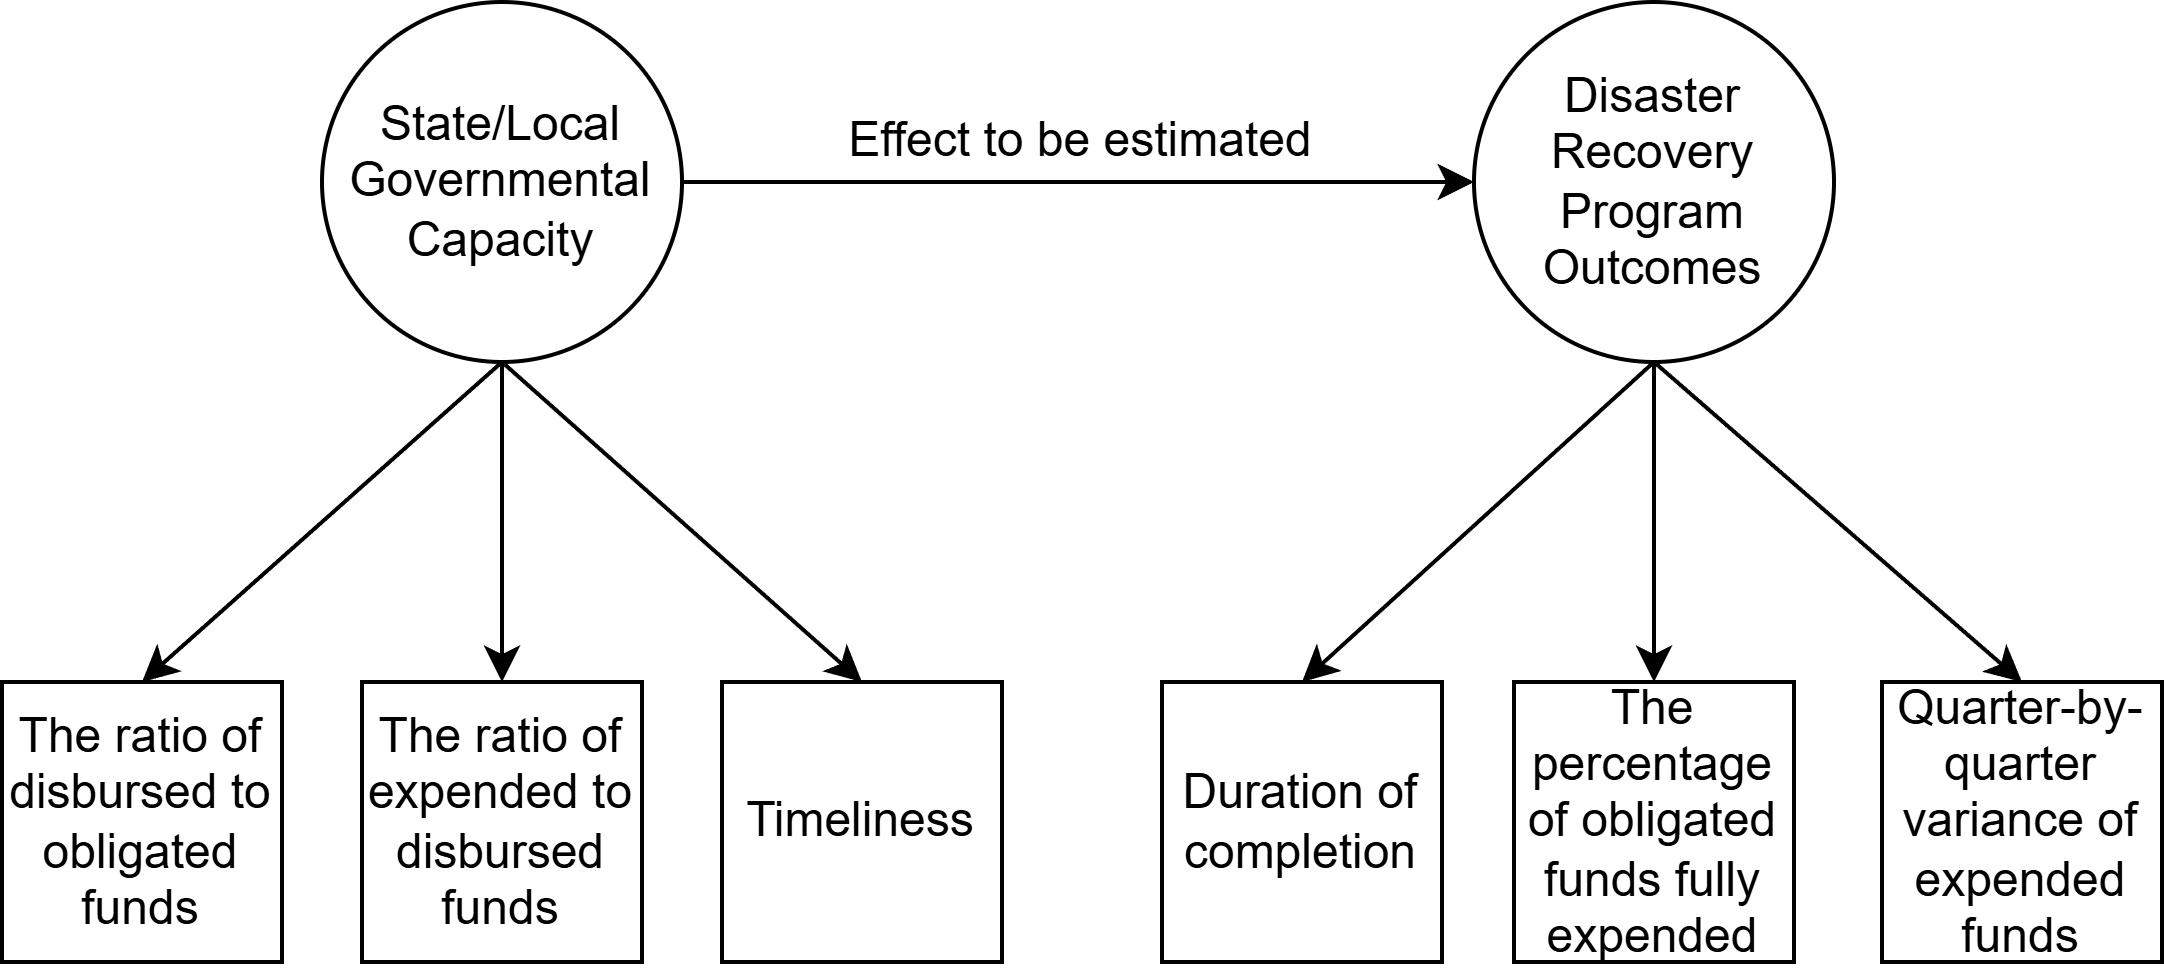
\includegraphics[keepaspectratio]{figures/fig_01_cross_sectional_sem.png}}

}

\caption{\label{fig-sem-conceptual}Structural equation model of
administrative throughput and disaster recovery outcomes.}

\end{figure}%

The SEM framework enables the analysis to distinguish between the
effects of greater administrative resources and those associated with
lower relative workload burdens. Both latent throughput dimensions are
specified as predictors of Recovery Performance and Recovery Timeliness
while controlling for governmental level, jurisdiction size, and the
four SVI dimensions. The two throughput dimensions are allowed to
covary, as are the two outcome constructs. These are modeled as direct
relationships rather than as interaction or moderation effects.

The measurement model defines the relationships between latent
constructs and their observed indicators:

\begin{itemize}
\tightlist
\item
  AdminResources \(\leftarrow\) avg\_employment, avg\_payroll
\item
  AdminBurdenCapacity \(\leftarrow\) rev\_programs\_per\_staff,
  rev\_disasters\_per\_staff
\item
  RecoveryPerformance \(\leftarrow\) ratio\_disbursed\_to\_obligated,
  ratio\_expended\_to\_disbursed,
  ratio\_total\_obligated\_funds\_fully\_expended,
  ratio\_program\_completed
\item
  RecoveryTimeliness \(\leftarrow\)
  rev\_duration\_of\_grant\_completion,
  rev\_average\_duration\_program\_completion
\end{itemize}

The structural model specifies the relationships between throughput,
control variables, and the latent outcome constructs:

\begin{itemize}
\tightlist
\item
  RecoveryPerformance \(\sim\) AdminResources + AdminBurdenCapacity +
  state\_or\_local + total\_population + SVI controls
\item
  RecoveryTimeliness \(\sim\) AdminResources + AdminBurdenCapacity +
  state\_or\_local + total\_population + SVI controls
\end{itemize}

The working expectation is that jurisdictions with greater
administrative resources and lower relative workload pressure will
exhibit stronger recovery outcomes. This expectation is treated as a
cross-sectional associational hypothesis rather than as a claim of
causal identification.

\subsection{Experimental Design and Model
Estimation}\label{experimental-design-and-model-estimation}

Two model-comparison and sensitivity strategies were implemented. First,
the analysis compares a two-factor SEM, in which Administrative
Resources and Administrative Burden Capacity are estimated separately,
with a one-factor SEM that combines all four indicators into a single
factor. Second, a smaller cleaned sample (N = 169) is documented for
provenance but is not used as a substantive robustness test because the
exact filtering rule cannot be reconstructed. Appendix Table A10 shows
that this subset is strictly contained within the 573-jurisdiction file
but does not correspond to any simple one-threshold outlier screen.

In the alternative one-factor SEM framework, the measurement model for a
single throughput factor (GovCapacity) is defined using all four
observed indicators: avg\_employment, avg\_payroll,
rev\_programs\_per\_staff, and rev\_disasters\_per\_staff, while the
measurement models for the disaster recovery outcome constructs remain
unchanged. The structural relationships are:

\begin{itemize}
\tightlist
\item
  RecoveryPerformance \(\sim\) GovCapacity + state\_or\_local +
  total\_population + SVI controls
\item
  RecoveryTimeliness \(\sim\) GovCapacity + state\_or\_local +
  total\_population + SVI controls
\end{itemize}

Prior to SEM estimation, all continuous indicators were standardized as
z-scores to improve comparability across variables and to support model
convergence, while the state\_level indicator remained coded 0/1. The
complete-case SEM input contains 573 jurisdictions and 17 variables with
no remaining missing values. The SEMs were estimated with conventional
maximum likelihood estimation (Lee \& Zhu, 2002), so the fit statistics,
standard errors, confidence intervals, and p-values reported here are
conventional ML quantities. Model evaluation relies on a combination of
fit statistics---chi-square, CFI, TLI, RMSEA, AIC, and BIC---rather than
on a single threshold. Model comparison is therefore treated as a
tradeoff exercise: the two-factor model is substantively more
informative and fits better on the main incremental and absolute fit
measures, while the one-factor model remains more parsimonious by
information criteria. Appendix Table A3 verifies the reported fit
statistics against reruns on the 573-jurisdiction SEM-ready dataset.

\section{Results}\label{results}

\subsection{SEM Model Comparison}\label{sem-model-comparison}

Both SEM specifications were estimated to examine the relationship
between administrative throughput and disaster recovery outcomes: (1) a
one-factor model in which all four throughput indicators load on a
single factor and (2) a two-factor model that separates Administrative
Resources from Administrative Burden Capacity.
Table~\ref{tbl-model-comparison} reports the comparison for the
573-jurisdiction complete-case SEM sample.

\begin{longtable}[]{@{}lrr@{}}
\caption{SEM model fit comparison. AIC and BIC are reported only for the
one-factor model because the two specifications use different numbers of
free parameters and the comparison is not straightforward on information
criteria alone.}\label{tbl-model-comparison}\tabularnewline
\toprule\noalign{}
Metric & One-Factor & Two-Factor \\
\midrule\noalign{}
\endfirsthead
\toprule\noalign{}
Metric & One-Factor & Two-Factor \\
\midrule\noalign{}
\endhead
\bottomrule\noalign{}
\endlastfoot
Chi-square (df) & 741.72 (101) & 469.82 (98) \\
Chi-square p-value & \textless{} 0.001 & \textless{} 0.001 \\
CFI & 0.854 & 0.915 \\
TLI & 0.818 & 0.891 \\
RMSEA & 0.105 & 0.081 \\
AIC & 67.41 & -- \\
BIC & 219.69 & -- \\
\end{longtable}

The model comparison reveals a genuine tradeoff rather than an
unambiguous winner. The one-factor model has lower information criteria
(AIC = 67.41; BIC = 219.69), but the two-factor model fits the
covariance structure more convincingly on the conventional SEM
diagnostics (CFI = 0.915 versus 0.854; TLI = 0.891 versus 0.818; RMSEA =
0.081 versus 0.105). Because the two-factor model aligns more closely
with the distinction between resources and workload as separate
dimensions of administrative throughput, and because it improves the
main fit indices materially, it is used as the primary substantive
model. At the same time, the one-factor alternative is more parsimonious
by AIC/BIC, so the two-factor model should be interpreted as preferred
conditionally rather than as definitively superior on every criterion.
Appendix Table A3 reports the fit-verification comparison.

The measurement parameters of the two-factor model also motivate a
cautious but interpretable reading. Within Administrative Resources,
standardized loadings are strong for employment (0.953) and payroll
(0.992). Within Administrative Burden Capacity, the reverse-coded
programs-per-staff indicator loads at 0.577 and disasters-per-staff
loads at approximately 1.000, indicating that the second factor is
driven more heavily by the disaster-workload component. Recovery
Performance is less coherent: disbursed-to-obligated loads at 0.785,
obligated funds fully expended at 0.988, programs completed at 0.477,
and expended-to-disbursed at \$-\$0.131. Recovery Timeliness is
identified by reverse-coded duration of completion (0.545) and
reverse-coded average program duration (1.000). The two latent
throughput dimensions are positively correlated (standardized covariance
= 0.402), and the structural part of the model explains more variance in
Recovery Timeliness than in Recovery Performance (approximate latent
\(R^2\) = 0.20 versus 0.09, based on standardized residual variances).
These features argue for interpreting the model as an exploratory
cross-sectional measurement structure rather than as a final, fully
settled confirmatory SEM. Recovery Timeliness is the more coherent and
policy-relevant outcome, whereas Recovery Performance is better treated
as a broader secondary summary. Appendix Tables A1, A2, A6, and A9
report the full measurement, structural, sensitivity, and
proxy-validation diagnostics.

\subsection{Structural Relationships Between Throughput and Recovery
Outcomes}\label{structural-relationships-between-throughput-and-recovery-outcomes}

The structural results indicate that Administrative Resources and
Administrative Burden Capacity relate to different recovery outcomes in
different ways. Table~\ref{tbl-structural} reports a highlighted subset
of the standardized structural path coefficients from the two-factor SEM
together with unstandardized 95\% confidence intervals. Appendix Table
A2 reports the full modeled path set, factor covariances, and residual
terms.

\begin{longtable}[]{@{}
  >{\raggedright\arraybackslash}p{(\linewidth - 8\tabcolsep) * \real{0.1364}}
  >{\raggedleft\arraybackslash}p{(\linewidth - 8\tabcolsep) * \real{0.2500}}
  >{\raggedleft\arraybackslash}p{(\linewidth - 8\tabcolsep) * \real{0.2273}}
  >{\raggedleft\arraybackslash}p{(\linewidth - 8\tabcolsep) * \real{0.1818}}
  >{\raggedleft\arraybackslash}p{(\linewidth - 8\tabcolsep) * \real{0.2045}}@{}}
\caption{Structural path estimates in the two-factor
SEM}\label{tbl-structural}\tabularnewline
\toprule\noalign{}
\begin{minipage}[b]{\linewidth}\raggedright
Path
\end{minipage} & \begin{minipage}[b]{\linewidth}\raggedleft
Std. Beta
\end{minipage} & \begin{minipage}[b]{\linewidth}\raggedleft
Unstd. b
\end{minipage} & \begin{minipage}[b]{\linewidth}\raggedleft
95\% CI
\end{minipage} & \begin{minipage}[b]{\linewidth}\raggedleft
p-value
\end{minipage} \\
\midrule\noalign{}
\endfirsthead
\toprule\noalign{}
\begin{minipage}[b]{\linewidth}\raggedright
Path
\end{minipage} & \begin{minipage}[b]{\linewidth}\raggedleft
Std. Beta
\end{minipage} & \begin{minipage}[b]{\linewidth}\raggedleft
Unstd. b
\end{minipage} & \begin{minipage}[b]{\linewidth}\raggedleft
95\% CI
\end{minipage} & \begin{minipage}[b]{\linewidth}\raggedleft
p-value
\end{minipage} \\
\midrule\noalign{}
\endhead
\bottomrule\noalign{}
\endlastfoot
AdminResources \(\to\) RecoveryPerformance & \$-\$0.170 &
\$-\(0.139 | [\)-\$0.212, \$-\$0.066{]} & \textless{} 0.001 & \\
AdminBurdenCapacity \(\to\) RecoveryPerformance & 0.077 & 0.104 &
{[}\$-\$0.015, 0.222{]} & 0.086 \\
AdminResources \(\to\) RecoveryTimeliness & 0.080 & 0.046 &
{[}\$-\$0.004, 0.095{]} & 0.072 \\
AdminBurdenCapacity \(\to\) RecoveryTimeliness & 0.266 & 0.251 &
{[}0.151, 0.352{]} & \textless{} 0.001 \\
SVI Theme 3 (Minority/Language) \(\to\) RecoveryPerformance & \$-\$0.226
& -- & -- & \textless{} 0.001 \\
SVI Theme 1 (Socioeconomic) \(\to\) RecoveryTimeliness & \$-\$0.194 & --
& -- & 0.004 \\
SVI Theme 2 (HH Comp./Disability) \(\to\) RecoveryTimeliness &
\$-\$0.159 & -- & -- & 0.004 \\
State-vs-Local \(\to\) RecoveryPerformance & \$-\$0.038 &
\$-\(0.133 | [\)-\$0.526, 0.259{]} & 0.505 & \\
State-vs-Local \(\to\) RecoveryTimeliness & \$-\$0.106 &
\$-\(0.260 | [\)-\$0.520, 0.000{]} & 0.050 & \\
\end{longtable}

\emph{Note}: Appendix Table A2 reports the complete modeled coefficient
set.

\subsubsection{Relationships with Recovery
Performance}\label{relationships-with-recovery-performance}

Administrative Resources exhibit a negative association with Recovery
Performance (\(\beta\) = \$-\$0.170; \(b\) = \$-\(0.139, 95% CI [
\)-\$0.212,
\$-\(0.066]; p < 0.001), indicating that jurisdictions with higher staffing and payroll intensity do not necessarily display stronger financial execution or program completion once workload pressure and contextual conditions are taken into account. This coefficient should not be read as evidence that more resources worsen recovery; at most it suggests that resource intensity may proxy for more complex portfolios or administrative settings that the pooled cross-sectional model does not fully observe. By contrast, Administrative Burden Capacity is positive but only marginally associated with Recovery Performance (\)\beta\$
= 0.077; \(b\) = 0.104, 95\% CI {[}\$-\$0.015, 0.222{]}; p = 0.086).
Manageable workload appears helpful for performance, but the evidence is
much stronger for timeliness.

Among the covariates, SVI Theme 3 (minority status and language
vulnerability) shows the clearest association with Recovery Performance
(\(\beta\) = \$-\$0.226, p \textless{} 0.001). This pattern should be
read as contextual rather than causal: jurisdictions serving more
linguistically diverse or historically marginalized communities may face
greater outreach, translation, verification, and service-delivery
demands, not because those communities cause weaker recovery, but
because administrative barriers and structural inequities can be harder
to overcome in those settings.

\subsubsection{Relationships with Recovery
Timeliness}\label{relationships-with-recovery-timeliness}

For Recovery Timeliness, Administrative Burden Capacity plays the
clearest role. Lower workload pressure relative to available staffing is
strongly associated with faster and more consistent recovery
implementation (\(\beta\) = 0.266; \(b\) = 0.251, 95\% CI {[}0.151,
0.352{]}; p \textless{} 0.001), indicating that administrative strain is
an important constraint on implementation speed. Administrative
Resources are positively associated with Recovery Timeliness as well,
but only marginally (\(\beta\) = 0.080; \(b\) = 0.046, 95\% CI
{[}\$-\$0.004, 0.095{]}; p = 0.072). This contrast reinforces the main
substantive message: resource levels matter, but workload manageability
appears to be the more consistent cross-sectional correlate of timely
recovery administration.

Two dimensions of social vulnerability are also significantly associated
with Recovery Timeliness. Higher values of SVI Theme 1 (socioeconomic
vulnerability) and SVI Theme 2 (household composition and disability)
are associated with slower implementation (\(\beta\) = \$-\$0.194, p =
0.004; \(\beta\) = \$-\$0.159, p = 0.004). The results suggest that
jurisdictions serving more socioeconomically vulnerable and
demographically constrained populations may face additional
administrative frictions that slow recovery even after throughput
proxies are taken into account.

The state-versus-local indicator is not statistically meaningful for
Recovery Performance (\(\beta\) =
\$-\(0.038; p = 0.505) and is only borderline negative for Recovery Timeliness (\)\beta\$
= \$-\$0.106; p = 0.050). Governmental level is therefore treated as a
control variable and a descriptive comparison device, not as a moderator
of throughput effects. The negative sign for timeliness suggests that
local governments may, on average, move somewhat faster than state
agencies once other covariates are controlled, but the evidence is too
modest and the institutional tasks too heterogeneous to support strong
claims about institutional superiority.

\subsubsection{SEM-Implied Relationship
Patterns}\label{sem-implied-relationship-patterns}

The SEM-implied predicted relationship plots further indicate that
Administrative Burden Capacity explains more of the visible variation in
recovery outcomes than Administrative Resources alone. The relationship
between workload manageability and both Recovery Performance and
Recovery Timeliness is upward, with the pattern appearing substantially
stronger for timeliness. These plots are useful visualization tools, but
they should not be interpreted as evidence of nonlinear causal effects;
they are derived from the fitted SEM and are best read as model-implied
association curves.

Administrative Resources exhibit a more complex relationship with
recovery outcomes. The negative coefficient for Recovery Performance may
reflect the fact that larger staffing and payroll footprints are
characteristic of more complex or higher-demand recovery portfolios.
Once workload is modeled explicitly, the resource indicators no longer
behave like simple monotonic measures of administrative effectiveness.

Most state agencies and local governments maintained relatively limited
staffing resources dedicated to administering CDBG-DR housing recovery
programs. As a result, the standardized values of both Administrative
Resources and Administrative Burden Capacity were concentrated near zero
for many jurisdictions, leading to more modest and sometimes less stable
marginal effects across recovery outcomes. This suggests that improving
recovery outcomes requires not only reducing administrative workload
pressures but also strengthening staffing and fiscal resources. However,
increasing administrative resources alone is insufficient to ensure
effective recovery implementation. Rather, enhancing throughput requires
a balanced combination of adequate resources and manageable program
demands.

\subsection{Spatial Patterns of Throughput and Recovery
Outcomes}\label{spatial-patterns-of-throughput-and-recovery-outcomes}

To complement the SEM results, we retain a small descriptive spatial
section showing how selected county-level throughput and recovery scores
are distributed geographically. These figures are not part of the SEM
estimation and are not used to establish additional statistical claims.
Instead, they provide visual context for whether the burden-throughput
pattern identified in the SEM appears concentrated in particular
regions.

Across the retained maps, the main descriptive pattern is
straightforward: workload manageability and Recovery Timeliness appear
more closely aligned than raw Administrative Resources and Recovery
Performance. Because these maps inherit values from county-linked and
state-agency profiles, they are best interpreted as secondary
descriptive context. The quadrant overlays and related county-level
summaries are retained as supplementary illustrations whose main value
is to show that the stronger burden-timeliness relationship is not
purely abstract when mapped descriptively. The gap diagnostics,
governance-risk screen, and exposure-capacity typologies are available
in the appendix for practitioners who may wish to use them as informal
screening tools.

\section{Discussion}\label{discussion}

\subsection{Rethinking Throughput: A Multi-Dimensional and Relational
Perspective}\label{rethinking-throughput-a-multi-dimensional-and-relational-perspective}

The results advance a more differentiated understanding of
administrative throughput in disaster recovery by showing that
throughput is not well captured by a single resource proxy. Across the
SEM and the limited descriptive spatial overlays, the most consistent
pattern is that recovery outcomes are more closely aligned with workload
manageability than with staffing and payroll intensity alone. That does
not mean resources are irrelevant; rather, it suggests that resources
must be interpreted relative to the disaster and program burdens they
are expected to absorb.

Consistent with Annan-Prah and Andoh (2023), we conceptualize throughput
as a joint reflection of resources and performance. However, we further
refine this perspective by introducing Administrative Burden Capacity,
defined as the effective throughput remaining after accounting for
workload pressures and contextual constraints such as social
vulnerability. This conceptualization highlights that throughput is
inherently relational: administrative resources only translate into
effective recovery outcomes when workload demands remain within
manageable levels.

A central contribution is the distinction between Administrative
Resources and Administrative Burden Capacity. Staffing and payroll
reflect the scale of the administrative system, whereas burden capacity
reflects how stretched that system is across disasters and programs. The
empirical evidence is strongest for Recovery Timeliness, where lower
workload pressure is associated with faster implementation. For Recovery
Performance, the burden-capacity path is positive but only marginal,
which suggests that the performance construct also reflects other
dimensions of organizational context, program design, and reporting
complexity. Burden capacity appears especially important for timing, and
plausibly relevant for performance, but not sufficient by itself to
explain all observed differences in recovery execution.

The negative association between Administrative Resources and Recovery
Performance further supports this interpretation. Rather than implying
that additional staff or payroll harms recovery, the coefficient likely
reflects portfolio complexity, organizational layering, or the fact that
more administratively intensive jurisdictions often manage more
demanding recovery contexts. Once workload is modeled explicitly, pure
resource intensity ceases to function as a simple proxy for
effectiveness. This result is therefore best treated as a potentially
confounded association that cautions against equating larger
bureaucratic scale with stronger recovery administration.

\subsection{Social Vulnerability and Spatial Inequality in Disaster
Recovery}\label{social-vulnerability-and-spatial-inequality-in-disaster-recovery}

The results also show that different dimensions of social vulnerability
relate to recovery outcomes through distinct channels. Minority status
and language vulnerability are most clearly associated with weaker
Recovery Performance, whereas socioeconomic vulnerability and household
composition/disability are more strongly associated with slower Recovery
Timeliness. One plausible interpretation is that vulnerability marks
contexts in which outreach, verification, coordination, and service
delivery barriers are harder to overcome. The SEM does not identify
those mechanisms directly, but the differentiated theme coefficients are
consistent with the idea that recovery governance becomes more difficult
when administrative burden and structural vulnerability overlap.

The limited spatial overlays are retained only as supplementary
screening tools. They may help show where workload pressure, exposure,
and vulnerability coincide, but they do not establish why those patterns
arise.

\subsection{Practical Implications}\label{practical-implications}

The findings provide decision-makers and practitioners with a more
nuanced understanding of throughput by distinguishing resource levels
from workload strain. For practice, the key implication is diagnostic:
when recovery performance is weak or implementation is slow, the problem
may not be simple resource scarcity. It may instead reflect the way
staffing, portfolio complexity, disaster exposure, and community
vulnerability interact. This perspective can help practitioners diagnose
whether recovery challenges stem from insufficient resources, excessive
administrative burden, or a broader misalignment between institutional
throughput and local recovery needs.

From a policy perspective, the results suggest that improving disaster
recovery outcomes requires moving beyond resource-centric approaches
toward workload-sensitive and context-aware interventions. Simply
increasing funding or staffing may have limited effect if administrative
systems remain overextended or if program complexity continues to impose
substantial procedural burden. More promising strategies may include
simplifying program rules, standardizing reporting and eligibility
workflows, deploying temporary surge-capacity teams during high-demand
periods (Khorram-Manesh, 2020), improving intergovernmental
coordination, and prioritizing high-risk jurisdictions for language
access, community outreach, and implementation support. These
recommendations remain associationally motivated rather than
experimentally verified, but they follow directly from the
burden-sensitive interpretation of the results.

Although the real-world effectiveness of these strategies requires
additional evaluation, the findings suggest that successful disaster
recovery depends not only on the amount of resources available but also
on whether those resources are adequate for the complexity, scale, and
vulnerability of the recovery environment in which they are deployed.

\subsection{Study Limitations}\label{study-limitations}

Several limitations should be acknowledged. First, the SEM relies on a
cross-sectional administering-jurisdiction dataset, so the results are
associational rather than causal. The aggregation from quarterly QPR
activity data to one profile per administering jurisdiction discards
within-jurisdiction variation across disasters, policy regimes, staffing
arrangements, and maturation windows. Appendix Table A5 makes that
maturity problem visible by showing that the sample spans markedly
different portfolio age bands. Second, the timeliness construct remains
duration-based and therefore sensitive to right-censoring and disaster
maturity. Newer grants and jurisdictions with ongoing portfolios have
had less time to complete recovery activities, which limits how strongly
the timeliness factor can be interpreted. The burden-timeliness
association reported here should therefore be characterized as
pooled-descriptive and maturity-sensitive rather than as a fully robust
structural relationship across all cohort compositions.

Third, the measurement of throughput remains indirect. QCEW NAICS 925110
employment and payroll are useful national proxies but do not directly
measure CDBG-DR administrative teams, contractors, or interagency
support structures. The workload indicators are likewise simplified
workload-density proxies rather than complete measures of administrative
strain. Appendix Tables A6, A7, and A9 report the sensitivity checks,
ratio-artifact diagnostics, and proxy-validation summaries, but these
remain partial validation steps rather than definitive proof that the
QCEW measures isolate true CDBG-DR staffing throughput. Similarly, the
SVI covariates are used as cross-sectional contextual controls rather
than as validated longitudinal trajectories.

Fourth, the geography layer is derived from hierarchical name matching
and county aggregation rather than from official Census relationship
files alone, even though the SEM sample labels resolve cleanly against
official 2023 Census state and county files. Fifth, the smaller cleaned
sensitivity sample remains only partially reconstructable; Appendix
Table A10 shows that it behaves like a compound or curated filter rather
than a simple outlier trim. Finally, the gap diagnostics and governance
risk index are descriptive composites rather than validated latent
constructs.

These limitations point to a clear future research agenda. Longitudinal
or event-history designs would address maturity and censoring more
directly. More detailed administrative-process data---such as staffing
assignments, contractor use, application processing times, and
intergovernmental coordination mechanisms---would make it possible to
move from proxy throughput measures toward more direct operational
indicators of recovery governance. Future work should also test narrower
cohorts or panel designs so that age of portfolio and disaster vintage
are separated more clearly from administrative throughput.

Despite these limitations, the analysis provides a useful empirical and
conceptual contribution. Across the SEM and the descriptive spatial
screens, the most consistent message is that disaster recovery
governance is shaped not simply by how many resources a jurisdiction
has, but by whether those resources are proportionate to disaster
workload and to the social conditions of implementation.

\section{Conclusion}\label{conclusion}

We develop an explicitly exploratory framework for examining
administrative throughput and disaster recovery outcomes across the
United States. Using pooled cross-sectional administering-jurisdiction
profiles, we move beyond purely resource-based indicators and evaluate
how staffing proxies, workload pressure, and contextual vulnerability
co-occur with Recovery Timeliness and, more tentatively, Recovery
Performance. The SEM provides the core evidence, while the gap
diagnostics and governance risk index serve as supplementary policy
screens.

Several key insights emerge. First, administrative throughput is not
well captured as a unidimensional construct. The two-factor model shows
that Administrative Resources and Administrative Burden Capacity behave
differently and should not be collapsed without checking the measurement
tradeoff. Second, the strongest throughput-outcome association in the
SEM is between lower workload pressure and faster Recovery Timeliness,
whereas the relationship with the broader Recovery Performance construct
is weaker and more conditional. Third, social vulnerability matters, but
different SVI themes relate to different parts of the recovery process,
reinforcing the view that throughput is embedded in broader
institutional and community contexts.

The limited descriptive spatial overlays add a geographic dimension to
those findings, but only in a supplementary sense. They help orient the
reader to where exposure, workload pressure, vulnerability, and weaker
outcomes may overlap, while remaining clearly secondary to the SEM.

Taken together, the analysis contributes conceptually by advancing a
workload-sensitive view of throughput, methodologically by making the
one-factor versus two-factor SEM tradeoff explicit, and practically by
showing that workload-sensitive diagnostic screening may be more useful
than simple staffing counts alone. The results should therefore be
interpreted as exploratory pooled cross-sectional associations, centered
on workload manageability and Recovery Timeliness, rather than as
definitive causal evidence about CDBG-DR recovery governance.

Improving disaster recovery governance (Tierney, 2012) will require more
than funding alone. It will require institutions whose staffing,
workload, and social context are better aligned with the scale and
complexity of recovery needs. The results provide an empirical starting
point for that discussion.

\section*{Acknowledgements}\label{acknowledgements}
\addcontentsline{toc}{section}{Acknowledgements}

This study is partially supported by funding from the U.S. Department of
Housing and Urban Development (Award\# H21749CA). The findings and
conclusions in this manuscript are those of the authors and do not
represent the official position or views of the U.S. Department of
Housing and Urban Development.

\section*{Disclosure Statement}\label{disclosure-statement}
\addcontentsline{toc}{section}{Disclosure Statement}

The authors declared no potential conflicts of interest with respect to
the research, authorship, and/or publication of this article. Generative
AI tools were used only for limited language editing. All analytic
decisions, interpretation, and manuscript content were reviewed and
approved by the authors.

\section*{Data Availability
Statement}\label{data-availability-statement}
\addcontentsline{toc}{section}{Data Availability Statement}

The public source datasets used in this study are HUD CDBG-DR DRGR/QPR
reports, U.S. Bureau of Labor Statistics QCEW files, and CDC/ATSDR SVI
data. The replication package for the published manuscript will include
the code, SEM-ready analytic data, derived geography linkage files, and
nonrestricted outputs needed to reproduce the reported models, tables,
and maps. Public source data will be cited directly, and any remaining
manually audited linkage notes will be provided as supplemental derived
documentation.

\section*{References}\label{references}
\addcontentsline{toc}{section}{References}

Annan-Prah, E. C., \& Andoh, R. P. K. (2023). Administrative capacity
and local level development in metropolitan, municipal and district
assemblies in Ghana: mediating role of resource capacity.
\emph{International Journal of Public Sector Management, 36}(3),
253--270.

CDC/ATSDR (Centers for Disease Control and Prevention / Agency for Toxic
Substances and Disease Registry). (2026). Geospatial Research, Analysis,
and Services Program. \emph{CDC/ATSDR Social Vulnerability Index 2022,
2020, 2018, 2016, 2014, 2010, \& 2000 Database U.S.}
https://www.atsdr.cdc.gov/placeandhealth/svi/data\_documentation\_download.html

Cevik, M. S., \& Huang, G. (2018). \emph{How to manage the fiscal costs
of natural disasters}. International Monetary Fund.

Costa, R., Mann, B., Sobhani, A., Hamideh, S., Nejat, A., \& Ross, A.
(2026). From Allocation to Action: A Comparative Analysis of CDBG-DR
Funding Expenditures for 2017 Disasters in California, Florida, and
Texas. \emph{SSRN preprint}.

Cutter, S. L., Ash, K. D., \& Emrich, C. T. (2016). Urban-rural
differences in disaster resilience. \emph{Annals of the American
Association of Geographers, 106}(6), 1236--1252.

Dzigbede, K. D., Gehl, S. B., \& Willoughby, K. (2020). Disaster
resiliency of US local governments: Insights to strengthen local
response and recovery from the COVID-19 pandemic. \emph{Public
Administration Review, 80}(4), 634--643.

El-Taliawi, O. G., \& Van Der Wal, Z. (2019). Developing administrative
capacity: An agenda for research and practice. \emph{Policy Design and
Practice, 2}(3), 243--257.

Geddam, S. M., Garg, P., \& Tyagi, A. (2024). Enhancing disaster
management effectiveness: A structural equation modeling approach.
\emph{International Journal of Disaster Risk Reduction, 99}, 104123.

Gendeshmin, S. B., Karami, S., \& Mousavi, S. M. (2025). Structural
equation modeling for disaster risk assessment: A systematic review.
\emph{International Journal of Disaster Risk Reduction, 119}, 105301.

Gigasheet. (2026). \emph{List of All U.S. Counties and Cities
Spreadsheet} (public lookup table used for preliminary city-to-county
matching).
https://www.gigasheet.com/sample-data/list-of-all-us-counties-and-cities-spreadsheet

Hamideh, S. (2015). \emph{Planning for disaster recovery: Lessons from
Hurricane Ike for theory and practice} (Doctoral dissertation). Texas
A\&M University.

Jordan, E., Javernick-Will, A., \& Amadei, B. (2014). A qualitative
comparative analysis of neighborhood recovery following Hurricane
Katrina. \emph{International Journal of Disaster Resilience in the Built
Environment, 5}(4), 391--412.

Khalid, S., \& Ashraf, I. (2024). The Role of Administrative Capacity in
Disaster Management. \emph{Social Trends and Policy Review, 2}(2),
97--133.

Khorram-Manesh, A. (2020). Flexible surge capacity---public health,
public education, and disaster management. \emph{Health Promotion
Perspectives, 10}(3), 175.

Kusumasari, B., Alam, Q., \& Siddiqui, K. (2010). Resource capability
for local government in managing disaster. \emph{Disaster Prevention and
Management, 19}(4), 438--451.

Lee, D. W. (2019). Local government's disaster management capacity and
disaster resilience. \emph{Local Government Studies, 45}(6), 803--826.

Lee, S. Y., \& Zhu, H. T. (2002). Maximum likelihood estimation of
nonlinear structural equation models. \emph{Psychometrika, 67}(2),
189--210.

Lindsay, B. R. (2014). \emph{FEMA's disaster relief fund: overview and
selected issues}. Congressional Research Service.

Martin, C. (2018). \emph{The Evidence Base on How CDBG-DR Works for
State and Local Stakeholders}. Urban Institute.

Martin, C., Gilbert, B., Teles, D., \& Theodos, B. (2019). \emph{Housing
Recovery and CDBG-DR}. Urban Institute.

Martin, C., Teles, D., \& DuBois, N. (2022). Understanding the pace of
HUD's disaster housing recovery efforts. \emph{Housing Policy Debate,
32}(1), 102--127.

Melendez, E. (2020). Puerto Rico Housing and Community Development
Industry's Capacity for Disaster Recovery. \emph{Centro Journal, 32}(3).

Miao, Q., Best, K., Reilly, A., \& Davlasheridze, M. (2025). Where Did
the Money Go? Assessing the Distribution of the Community Development
Block Grant-Disasters Recovery Funds. \emph{The American Review of
Public Administration, 55}(3), 227--248.

Nor, M. I. (2025). Investigating the dynamics of climate finance
disbursements: A panel data approach from 2003 to 2022. \emph{PLOS One,
20}(3), e0318170.

Ospina, S. M., Esteve, M., \& Lee, S. (2018). Assessing qualitative
studies in public administration research. \emph{Public Administration
Review, 78}(4), 593--605.

Peacock, W. G., Van Zandt, S., Zhang, Y., \& Highfield, W. E. (2014).
Inequities in long-term housing recovery after disasters. \emph{Journal
of the American Planning Association, 80}(4), 356--371.

Rosas, E., Roberts, P. S., Lauland, A., Gutierrez, I. A., \& Nunez-Neto,
B. (2021). Assessing the impact of municipal government capacity on
recovery from Hurricane Maria in Puerto Rico. \emph{International
Journal of Disaster Risk Reduction, 61}, 102340.

Rouhanizadeh, B., Kermanshachi, S., \& Nipa, T. J. (2020). Exploratory
analysis of barriers to effective post-disaster recovery.
\emph{International Journal of Disaster Risk Reduction, 50}, 101735.

Rouhanizadeh, B., Kermanshachi, S., \& Safapour, E. (2022). An
investigation of causal relationships among barriers that delay
post-hurricane recovery of human communities. \emph{International
Journal of Disaster Risk Reduction, 67}, 102666.

Safapour, E., Kermanshachi, S., \& Pamidimukkala, A. (2021).
Post-disaster recovery in urban and rural communities: Challenges and
strategies. \emph{International Journal of Disaster Risk Reduction, 64},
102535.

Tierney, K. (2012). Disaster governance: Social, political, and economic
dimensions. \emph{Annual Review of Environment and Resources, 37},
341--363.

U.S. Bureau of Labor Statistics. (2026). \emph{Quarterly Census of
Employment and Wages}.
https://www.bls.gov/cew/downloadable-data-files.htm

U.S. Department of Housing and Urban Development. (2026). \emph{CDBG-DR
Reports}. https://www.hud.gov/hud-partners/community-cdbg-dr-reports

U.S. Government Accountability Office. (2019). \emph{Disaster recovery:
Better monitoring of block grant funds is needed}.
https://www.gao.gov/products/gao-19-232

Van Niekerk, D., Nemakonde, L. D., Kruger, L., \& Forbes-Genade, K.
(2018). Community-Based Disaster Risk Management. In H. Rodriguez, W.
Donner, \& J. Trainor (Eds.), \emph{Handbook of Disaster Research}.
Springer.

\newpage

\section*{Appendix A: Data Description and
Provenance}\label{appendix-a-data-description-and-provenance}
\addcontentsline{toc}{section}{Appendix A: Data Description and
Provenance}

\subsection{A.1 Source Data}\label{a.1-source-data}

The empirical results reported in this paper come from three data
sources: the standardized QPR data (\texttt{qpr\_standardized.parquet}),
containing 130,605 activity-quarter rows; the grantee-disaster feature
panel (\texttt{panel\_features.parquet}); and manuscript-specific
robustness tables stored in the diagnostics directory.

The standardized QPR data contain one row per activity within a
grantee-disaster-quarter, not one row per quarter. The cross-sectional
SEM does not estimate on this file directly. Instead, the feature
pipeline collapses the QPR records to a grantee-disaster panel of 156
observations and then, for the cross-sectional SEM, to one mean profile
per administering jurisdiction.

\subsection{A.2 Transformation Chain}\label{a.2-transformation-chain}

The transformation chain relevant to the SEM is as follows. First, QPR
raw exports are cleaned and standardized into quarter-aware records.
Second, grantee-disaster features are computed, including financial
ratios and timing summaries. Third, a censoring rule is applied for one
specification: Duration\_censored equals the number of observed quarters
whenever 95 percent completion is not reached. Fourth, the same
specification defines Timeliness\_censored as the inverse of
Duration\_censored. Fifth, the cross-sectional SEM aggregates
grantee-disaster measures to the administering-jurisdiction level using
means. The positive structural path in the full 3x3 model appears only
after steps three through five. The main body of the paper therefore
treats those steps as objects of methodological scrutiny rather than as
innocuous preprocessing choices.

\subsection{A.3 Sample Sizes}\label{a.3-sample-sizes}

The main sample counts used in the analysis are reported in
Table~\ref{tbl-sample-sizes}.

\begin{longtable}[]{@{}
  >{\raggedright\arraybackslash}p{(\linewidth - 4\tabcolsep) * \real{0.3000}}
  >{\raggedleft\arraybackslash}p{(\linewidth - 4\tabcolsep) * \real{0.4000}}
  >{\raggedright\arraybackslash}p{(\linewidth - 4\tabcolsep) * \real{0.3000}}@{}}
\caption{Sample sizes used in the
analysis}\label{tbl-sample-sizes}\tabularnewline
\toprule\noalign{}
\begin{minipage}[b]{\linewidth}\raggedright
Sample
\end{minipage} & \begin{minipage}[b]{\linewidth}\raggedleft
N
\end{minipage} & \begin{minipage}[b]{\linewidth}\raggedright
Notes
\end{minipage} \\
\midrule\noalign{}
\endfirsthead
\toprule\noalign{}
\begin{minipage}[b]{\linewidth}\raggedright
Sample
\end{minipage} & \begin{minipage}[b]{\linewidth}\raggedleft
N
\end{minipage} & \begin{minipage}[b]{\linewidth}\raggedright
Notes
\end{minipage} \\
\midrule\noalign{}
\endhead
\bottomrule\noalign{}
\endlastfoot
Grantee-disaster feature panel & 156 & All grantee-disaster pairs in the
working panel \\
Unique administering jurisdictions & 78 & Cross-sectional aggregation
target \\
Disaster types & 18 & Disaster contexts represented in the panel \\
Full and reduced SEM complete cases & 41 & Overall cross-sectional SEM
sample \\
Non-circular baseline SEM & 40 & Overall baseline cross-sectional SEM
sample \\
State subset & 23 & Complete cases in subset comparison \\
Local subset & 17 & Complete cases in subset comparison \\
Full 3x3 state replication & 36 & Grantee-level state sample after
censoring and aggregation \\
\end{longtable}

These counts represent complete-case estimation samples, not the total
information available in the QPR data.

\subsection{A.4 Timing and Maturity
Limits}\label{a.4-timing-and-maturity-limits}

The analysis covers disaster cohorts from 2003 through 2023. The
standardized QPR data contain quarterly observations from September 2002
through June 2025. The absolute dates matter because the 95 percent
completion rule is maturity-sensitive: more recent disasters have had
fewer reporting quarters in which to approach the completion threshold,
making duration-based outcomes vulnerable to right-censoring and cohort
bias.

The data processing pipeline applies a minimum-quarter filter and ratio
winsorization to reduce extreme values. Only those preprocessing rules
that can be traced in the data pipeline are reported; no additional
outlier-deletion procedure is claimed.

\subsection{A.5 External Data Sources}\label{a.5-external-data-sources}

The analysis in the main body uses financial-flow indicators derived
from QPR data. Additional external sources that could extend this
framework include BLS QCEW staffing and payroll measures (NAICS 925110),
CDC/ATSDR Social Vulnerability Index vintages, and city-to-county
geography matching. The QCEW and SVI data are used in the
573-jurisdiction SEM specification reported in the main text. If future
work reintroduces additional external variables, the following
documentation would be needed: for QCEW, extraction year coverage,
suppression handling, and a clear statement that NAICS 925110 is an
indirect proxy rather than a direct staff count; for SVI, either a
harmonization protocol across vintages or a design that avoids direct
comparison of percentile scores across incompatible releases; for
geography matching, a source hierarchy, match shares by method,
unresolved cases, and validation against official Census relationship
files.

\subsection{A.6 Data Availability
Categories}\label{a.6-data-availability-categories}

For the purposes of replication, the data fall into three categories:
public raw sources (HUD DRGR/QPR administrative exports, Census
population series, BLS QCEW, CDC/ATSDR SVI); shareable derivative
materials (analysis code, robustness tables, and nonrestricted outputs);
and controlled materials (any historical manual linkage tables or
geography crosswalks that would require a separate curation pass before
distribution).

\newpage

\section*{Appendix B: Methodological
Details}\label{appendix-b-methodological-details}
\addcontentsline{toc}{section}{Appendix B: Methodological Details}

\subsection{B.1 SEM Specification
Families}\label{b.1-sem-specification-families}

Three classes of SEM specification are compared. In all cases, the
measurement model is treated as an exploratory latent summary rather
than a confirmed reflective structure. The indicators may function as
formative components (determinants of throughput) rather than reflective
manifestations (effects of a latent trait), and the specifications
adopted here do not distinguish between these alternatives.

The \emph{full 3x3 models} use censored duration and inverse-duration
timeliness as indicators. The \emph{non-circular baseline models} remove
the deterministic overlap between throughput and outcome timing
indicators. The \emph{alternative indicator models}, including milestone
and duration-free variants, are used only for sensitivity checks. No
moderation model is estimated. State-versus-local results are subset
comparisons, not interaction tests, multi-group invariance analyses, or
moderation estimates.

\subsection{B.2 Full 3x3 Versus Non-Circular
Baseline}\label{b.2-full-3x3-versus-non-circular-baseline}

The full 3x3 specification is:

\[
\text{gov\_cap} =\!\sim \text{Ratio\_disbursed\_to\_obligated} + \text{Ratio\_expended\_to\_disbursed} + \text{Timeliness\_censored}
\]

\[
\text{recovery\_outcome} =\!\sim \text{Duration\_censored} + \text{Ratio\_obligated\_funds\_fully\_expended} + \text{Quarter\_by\_quarter\_variance\_expended}
\]

\[
\text{recovery\_outcome} \sim \text{gov\_cap}
\]

The preferred non-circular baseline is:

\[
\text{gov\_cap} =\!\sim \text{Ratio\_disbursed\_to\_obligated} + \text{Ratio\_expended\_to\_disbursed}
\]

\[
\text{recovery\_outcome} =\!\sim \text{Duration\_log} + \text{Spending\_CV}
\]

\[
\text{recovery\_outcome} \sim \text{gov\_cap}
\]

The non-circular baseline is preferred because it avoids the
timeliness-duration coupling described in Section B.3. It is not
presented as a well-validated measurement model but rather as the least
problematic available specification.

\subsection{B.3 Why the Timing Construction Is
Problematic}\label{b.3-why-the-timing-construction-is-problematic}

The full 3x3 specification defines:

\[
\text{Duration\_censored}_i =
\begin{cases}
\text{Duration}_i, & \text{if 95\% completion is observed} \\
\text{N\_Quarters}_i, & \text{otherwise}
\end{cases}
\]

and then

\[
\text{Timeliness\_censored}_i = \frac{1}{\text{Duration\_censored}_i}
\]

A single underlying duration quantity therefore enters the SEM twice:
once directly on the outcome factor and once inversely on the throughput
factor. The large positive structural path in the full 3x3 model cannot
be treated as clean evidence for an underlying throughput effect because
of this mathematical coupling.

\subsection{B.4 Available Measurement
Evidence}\label{b.4-available-measurement-evidence}

Parameter tables are available for selected specifications but do not
constitute a complete package of residual matrices, construct
reliability statistics, or standardized latent-correlation tables for
every model. The tables below report what is available; missing elements
are treated as a methodological limitation.

\subsubsection{Non-Circular Baseline: Loadings and Structural Path (All
Jurisdictions)}\label{non-circular-baseline-loadings-and-structural-path-all-jurisdictions}

\begin{longtable}[]{@{}lrrr@{}}
\toprule\noalign{}
Parameter & Estimate & Standard error & p-value \\
\midrule\noalign{}
\endhead
\bottomrule\noalign{}
\endlastfoot
recovery\_outcome \textasciitilde{} gov\_cap & 0.320 & 6.137 & 0.958 \\
Ratio\_expended\_to\_disbursed \textasciitilde{} gov\_cap & \$-\$0.102 &
1.977 & 0.959 \\
Spending\_CV \textasciitilde{} recovery\_outcome & \$-\$0.367 & 2.174 &
0.866 \\
\end{longtable}

\subsubsection{Full 3x3 State
Replication}\label{full-3x3-state-replication}

\begin{longtable}[]{@{}
  >{\raggedright\arraybackslash}p{(\linewidth - 6\tabcolsep) * \real{0.2000}}
  >{\raggedleft\arraybackslash}p{(\linewidth - 6\tabcolsep) * \real{0.2667}}
  >{\raggedleft\arraybackslash}p{(\linewidth - 6\tabcolsep) * \real{0.2667}}
  >{\raggedleft\arraybackslash}p{(\linewidth - 6\tabcolsep) * \real{0.2667}}@{}}
\toprule\noalign{}
\begin{minipage}[b]{\linewidth}\raggedright
Parameter
\end{minipage} & \begin{minipage}[b]{\linewidth}\raggedleft
Estimate
\end{minipage} & \begin{minipage}[b]{\linewidth}\raggedleft
Standard error
\end{minipage} & \begin{minipage}[b]{\linewidth}\raggedleft
p-value
\end{minipage} \\
\midrule\noalign{}
\endhead
\bottomrule\noalign{}
\endlastfoot
recovery\_outcome \textasciitilde{} gov\_cap & 113.652 & 17.535 &
\textless{} 0.001 \\
Ratio\_expended\_to\_disbursed \textasciitilde{} gov\_cap & 1.254 &
1.305 & 0.337 \\
Timeliness\_censored \textasciitilde{} gov\_cap & \$-\$0.273 & 0.075 &
\textless{} 0.001 \\
Ratio\_obligated\_funds\_fully\_expended \textasciitilde{}
recovery\_outcome & 0.0106 & 0.0011 & \textless{} 0.001 \\
Quarter\_by\_quarter\_variance\_expended \textasciitilde{}
recovery\_outcome & \$-\$0.0001 & 0.0006 & 0.831 \\
\end{longtable}

These tables illustrate why the full 3x3 result appears strong and why
the non-circular baseline does not. They are not sufficient to claim
full construct validation. A rigorous measurement validation would
require confirmatory factor analysis on a hold-out sample with adequate
power (conventionally N \textgreater{} 200 per group), comparison of
reflective versus formative specifications using MIMIC or PLS-SEM, and
convergent and discriminant validity testing against external indicators
such as staffing levels or prior program experience. None of these steps
were feasible given the available complete-case samples (N = 40 overall,
N = 23 state, N = 17 local).

\subsection{B.5 Fit Interpretation}\label{b.5-fit-interpretation}

Fit indices are reported as estimated, with two cautions. First, very
small SEM samples with low degrees of freedom can produce unstable or
non-intuitive fit values, including CFI or TLI estimates above 1.0.
Second, no model satisfies a clean combination of strong incremental
fit, acceptable absolute fit, and conceptually non-overlapping
indicators. For this reason, no single specification is declared a
preferred confirmatory measurement model; the comparison table in the
main text documents the tradeoffs across specifications.

\subsection{B.6 Excluded Metrics}\label{b.6-excluded-metrics}

Administrative gap measures and a Recovery Governance Risk Index are
referenced in the spatial sections of the main text as descriptive
screening tools. These composites are not estimated as part of the SEM
and are not treated as validated latent constructs. Their construction
is documented in the replication materials rather than in the main text.

\subsection{B.7 Interpretation Rule}\label{b.7-interpretation-rule}

All throughput-outcome relationships are interpreted as associational
and exploratory. The analysis does not claim moderation, causal
identification, or stable state-versus-local effect heterogeneity.

\newpage

\section*{Appendix C: Robustness
Tables}\label{appendix-c-robustness-tables}
\addcontentsline{toc}{section}{Appendix C: Robustness Tables}

\subsection{C.1 Specification
Comparison}\label{c.1-specification-comparison}

Table~\ref{tbl-spec-comparison} reports fit indices across six SEM
specifications estimated on the cross-sectional sample described in the
main text.

\begin{longtable}[]{@{}
  >{\raggedright\arraybackslash}p{(\linewidth - 16\tabcolsep) * \real{0.0857}}
  >{\raggedleft\arraybackslash}p{(\linewidth - 16\tabcolsep) * \real{0.1143}}
  >{\raggedleft\arraybackslash}p{(\linewidth - 16\tabcolsep) * \real{0.1143}}
  >{\raggedleft\arraybackslash}p{(\linewidth - 16\tabcolsep) * \real{0.1143}}
  >{\raggedleft\arraybackslash}p{(\linewidth - 16\tabcolsep) * \real{0.1143}}
  >{\raggedleft\arraybackslash}p{(\linewidth - 16\tabcolsep) * \real{0.1143}}
  >{\raggedleft\arraybackslash}p{(\linewidth - 16\tabcolsep) * \real{0.1143}}
  >{\raggedleft\arraybackslash}p{(\linewidth - 16\tabcolsep) * \real{0.1143}}
  >{\raggedleft\arraybackslash}p{(\linewidth - 16\tabcolsep) * \real{0.1143}}@{}}
\caption{Specification comparison across SEM
models}\label{tbl-spec-comparison}\tabularnewline
\toprule\noalign{}
\begin{minipage}[b]{\linewidth}\raggedright
Model
\end{minipage} & \begin{minipage}[b]{\linewidth}\raggedleft
\(\chi^2\)
\end{minipage} & \begin{minipage}[b]{\linewidth}\raggedleft
\(\chi^2\) p-value
\end{minipage} & \begin{minipage}[b]{\linewidth}\raggedleft
CFI
\end{minipage} & \begin{minipage}[b]{\linewidth}\raggedleft
TLI
\end{minipage} & \begin{minipage}[b]{\linewidth}\raggedleft
RMSEA
\end{minipage} & \begin{minipage}[b]{\linewidth}\raggedleft
AIC
\end{minipage} & \begin{minipage}[b]{\linewidth}\raggedleft
BIC
\end{minipage} & \begin{minipage}[b]{\linewidth}\raggedleft
N
\end{minipage} \\
\midrule\noalign{}
\endfirsthead
\toprule\noalign{}
\begin{minipage}[b]{\linewidth}\raggedright
Model
\end{minipage} & \begin{minipage}[b]{\linewidth}\raggedleft
\(\chi^2\)
\end{minipage} & \begin{minipage}[b]{\linewidth}\raggedleft
\(\chi^2\) p-value
\end{minipage} & \begin{minipage}[b]{\linewidth}\raggedleft
CFI
\end{minipage} & \begin{minipage}[b]{\linewidth}\raggedleft
TLI
\end{minipage} & \begin{minipage}[b]{\linewidth}\raggedleft
RMSEA
\end{minipage} & \begin{minipage}[b]{\linewidth}\raggedleft
AIC
\end{minipage} & \begin{minipage}[b]{\linewidth}\raggedleft
BIC
\end{minipage} & \begin{minipage}[b]{\linewidth}\raggedleft
N
\end{minipage} \\
\midrule\noalign{}
\endhead
\bottomrule\noalign{}
\endlastfoot
Full 3x3 & 15.384 & 0.052 & 0.938 & 0.883 & 0.152 & 25.250 & 47.526 &
41 \\
Reduced & 56.315 & \textless{} 0.001 & 0.498 & \$-\$0.256 & 0.572 &
19.253 & 38.102 & 41 \\
Non-circular baseline & 0.022 & 0.882 & 0.790 & \$-\$0.259 & 0.000 &
17.999 & 33.199 & 40 \\
Non-circular variant & 2.710 & 0.608 & 0.758 & 0.394 & 0.000 & 21.865 &
40.442 & 40 \\
Improved 3x3 & 4.094 & 0.848 & 1.486 & 1.911 & 0.000 & 25.795 & 47.751 &
40 \\
Improved 3x3 (progress) & 57.005 & \textless{} 0.001 & 0.238 &
\$-\$0.430 & 0.396 & 23.150 & 45.105 & 40 \\
\end{longtable}

\subsection{C.2 State and Local Subset
Comparison}\label{c.2-state-and-local-subset-comparison}

Table~\ref{tbl-subset-comparison} reports fit indices for the
non-circular baseline specification estimated separately on all
jurisdictions, state jurisdictions, and local jurisdictions. These
subset results are sensitivity checks; the fit values are too unstable
for strong inference, and the sample sizes are too small to support a
formal state-versus-local comparison.

\begin{longtable}[]{@{}
  >{\raggedright\arraybackslash}p{(\linewidth - 16\tabcolsep) * \real{0.0857}}
  >{\raggedleft\arraybackslash}p{(\linewidth - 16\tabcolsep) * \real{0.1143}}
  >{\raggedleft\arraybackslash}p{(\linewidth - 16\tabcolsep) * \real{0.1143}}
  >{\raggedleft\arraybackslash}p{(\linewidth - 16\tabcolsep) * \real{0.1143}}
  >{\raggedleft\arraybackslash}p{(\linewidth - 16\tabcolsep) * \real{0.1143}}
  >{\raggedleft\arraybackslash}p{(\linewidth - 16\tabcolsep) * \real{0.1143}}
  >{\raggedleft\arraybackslash}p{(\linewidth - 16\tabcolsep) * \real{0.1143}}
  >{\raggedleft\arraybackslash}p{(\linewidth - 16\tabcolsep) * \real{0.1143}}
  >{\raggedleft\arraybackslash}p{(\linewidth - 16\tabcolsep) * \real{0.1143}}@{}}
\caption{Subset fit comparison for the non-circular
baseline}\label{tbl-subset-comparison}\tabularnewline
\toprule\noalign{}
\begin{minipage}[b]{\linewidth}\raggedright
Subset
\end{minipage} & \begin{minipage}[b]{\linewidth}\raggedleft
\(\chi^2\)
\end{minipage} & \begin{minipage}[b]{\linewidth}\raggedleft
\(\chi^2\) p-value
\end{minipage} & \begin{minipage}[b]{\linewidth}\raggedleft
CFI
\end{minipage} & \begin{minipage}[b]{\linewidth}\raggedleft
TLI
\end{minipage} & \begin{minipage}[b]{\linewidth}\raggedleft
RMSEA
\end{minipage} & \begin{minipage}[b]{\linewidth}\raggedleft
AIC
\end{minipage} & \begin{minipage}[b]{\linewidth}\raggedleft
BIC
\end{minipage} & \begin{minipage}[b]{\linewidth}\raggedleft
N
\end{minipage} \\
\midrule\noalign{}
\endfirsthead
\toprule\noalign{}
\begin{minipage}[b]{\linewidth}\raggedright
Subset
\end{minipage} & \begin{minipage}[b]{\linewidth}\raggedleft
\(\chi^2\)
\end{minipage} & \begin{minipage}[b]{\linewidth}\raggedleft
\(\chi^2\) p-value
\end{minipage} & \begin{minipage}[b]{\linewidth}\raggedleft
CFI
\end{minipage} & \begin{minipage}[b]{\linewidth}\raggedleft
TLI
\end{minipage} & \begin{minipage}[b]{\linewidth}\raggedleft
RMSEA
\end{minipage} & \begin{minipage}[b]{\linewidth}\raggedleft
AIC
\end{minipage} & \begin{minipage}[b]{\linewidth}\raggedleft
BIC
\end{minipage} & \begin{minipage}[b]{\linewidth}\raggedleft
N
\end{minipage} \\
\midrule\noalign{}
\endhead
\bottomrule\noalign{}
\endlastfoot
All jurisdictions & 0.022 & 0.882 & 0.790 & \$-\$0.259 & 0.000 & 17.999
& 33.199 & 40 \\
State jurisdictions & 2.134 & 0.144 & 1.379 & 3.276 & 0.227 & 17.814 &
28.034 & 23 \\
Local jurisdictions & 2.209 & 0.137 & 1.372 & 3.233 & 0.275 & 17.740 &
25.239 & 17 \\
\end{longtable}

\subsection{C.3 Alternative Outcome
Specifications}\label{c.3-alternative-outcome-specifications}

Table~\ref{tbl-alt-outcomes} reports structural path estimates from
alternative outcome specifications that avoid the timeliness-duration
coupling present in the full 3x3 model. Across all alternative designs,
the non-circular SEMs remain non-significant. Expanding the sample
through duration-free or milestone-based outcomes does not recover a
stable positive throughput effect.

\begin{longtable}[]{@{}
  >{\raggedright\arraybackslash}p{(\linewidth - 12\tabcolsep) * \real{0.1154}}
  >{\raggedright\arraybackslash}p{(\linewidth - 12\tabcolsep) * \real{0.1154}}
  >{\raggedleft\arraybackslash}p{(\linewidth - 12\tabcolsep) * \real{0.1538}}
  >{\raggedleft\arraybackslash}p{(\linewidth - 12\tabcolsep) * \real{0.1538}}
  >{\raggedleft\arraybackslash}p{(\linewidth - 12\tabcolsep) * \real{0.1538}}
  >{\raggedleft\arraybackslash}p{(\linewidth - 12\tabcolsep) * \real{0.1538}}
  >{\raggedleft\arraybackslash}p{(\linewidth - 12\tabcolsep) * \real{0.1538}}@{}}
\caption{Alternative outcome
specifications}\label{tbl-alt-outcomes}\tabularnewline
\toprule\noalign{}
\begin{minipage}[b]{\linewidth}\raggedright
Model
\end{minipage} & \begin{minipage}[b]{\linewidth}\raggedright
Subset
\end{minipage} & \begin{minipage}[b]{\linewidth}\raggedleft
N
\end{minipage} & \begin{minipage}[b]{\linewidth}\raggedleft
CFI
\end{minipage} & \begin{minipage}[b]{\linewidth}\raggedleft
RMSEA
\end{minipage} & \begin{minipage}[b]{\linewidth}\raggedleft
Throughput \(\beta\)
\end{minipage} & \begin{minipage}[b]{\linewidth}\raggedleft
p-value
\end{minipage} \\
\midrule\noalign{}
\endfirsthead
\toprule\noalign{}
\begin{minipage}[b]{\linewidth}\raggedright
Model
\end{minipage} & \begin{minipage}[b]{\linewidth}\raggedright
Subset
\end{minipage} & \begin{minipage}[b]{\linewidth}\raggedleft
N
\end{minipage} & \begin{minipage}[b]{\linewidth}\raggedleft
CFI
\end{minipage} & \begin{minipage}[b]{\linewidth}\raggedleft
RMSEA
\end{minipage} & \begin{minipage}[b]{\linewidth}\raggedleft
Throughput \(\beta\)
\end{minipage} & \begin{minipage}[b]{\linewidth}\raggedleft
p-value
\end{minipage} \\
\midrule\noalign{}
\endhead
\bottomrule\noalign{}
\endlastfoot
Duration-free CV & All & 156 & 0.990 & 0.105 & 0.360 & 0.132 \\
Duration-free CV & State & 94 & 0.979 & 0.163 & 0.326 & 0.179 \\
Duration-free CV & Local & 61 & 0.968 & 0.164 & 0.337 & 0.431 \\
Milestone: time to 50\% & All & 156 & 0.758 & 0.308 & \$-\$0.365 &
0.354 \\
Milestone: time to 50\% & State & 94 & 0.983 & 0.093 & \$-\$0.442 &
0.404 \\
Milestone: time to 50\% & Local & 61 & 0.691 & 0.434 & \$-\$0.266 &
0.617 \\
Milestone: progress rate & All & 156 & 0.847 & 0.092 & 0.091 & 0.685 \\
Milestone: velocity & All & 156 & 0.995 & 0.209 & 0.014 & 0.669 \\
\end{longtable}

\subsection{C.4 Outlier and Preprocessing
Sensitivity}\label{c.4-outlier-and-preprocessing-sensitivity}

Winsorization and trimming of extreme ratio values are applied during
preprocessing. No additional outlier-removal robustness pass beyond
those preprocessing steps is claimed. The robustness evidence should be
treated as limited to the specification, subset, and alternative outcome
tables reported here.

\subsection{C.5 Summary}\label{c.5-summary}

The robustness evidence points in one direction: the large positive SEM
path appears only in the full 3x3 specification that uses censored
duration and its inverse as timeliness. Once the timing overlap is
removed or the outcome is redefined, the structural path is no longer
statistically persuasive.




\end{document}
